\documentclass[11pt,a4paper]{article}
\usepackage[utf8]{inputenc}
\usepackage[T1]{fontenc}
\usepackage{lmodern}
\usepackage{geometry}
\geometry{margin=1in}

\usepackage{amsmath,amssymb}
\usepackage{graphicx}
\usepackage{booktabs}
\usepackage{caption}
\usepackage{subcaption}
\usepackage{hyperref}
\usepackage{xcolor}
\usepackage{float}

\title{Face Recognition Lab: PCA Dimensionality Reduction with K-Means and GMM Clustering}
\author{
   Youssef Khamis : 22011381\\
   Muhnad Sayed : 22011902\\
   Ali Eldeen Maher : 22010934
}
\date{\today}

\begin{document}
\maketitle

\begin{abstract}
This report studies facial image representation using Principal Component Analysis (PCA) and compares two unsupervised classifiers---K-Means clustering and Gaussian Mixture Models (GMM)---on PCA-reduced features. We sweep the PCA variance threshold $\alpha$ and the number of clusters $K$ to analyze how they affect classification performance. Evaluation is performed on a held-out test set using clustering accuracy, weighted F1-score, and confusion matrices. All experiments are run with fixed random seed 42 for reproducibility.
\end{abstract}

\section{Introduction}
Face recognition can be approached by learning a compact representation of face images and then performing classification in that low-dimensional space. PCA provides a classic linear dimensionality reduction method (``eigenfaces'') that captures the most significant directions of variance in the dataset. After projection into the PCA subspace, we can apply unsupervised clustering methods. To measure recognition performance with class labels available, we map each cluster to a subject label using the training set.

\section{Dataset and Experimental Setup}
\subsection{Data}
We use a face dataset where each sample is a grayscale image vectorized into a feature vector (pixel intensities). The data is split into training set $(X_{\text{train}}, y_{\text{train}})$ and test set $(X_{\text{test}}, y_{\text{test}})$.

\subsection{Reproducibility}
A fixed random seed is used throughout the lab:
\begin{equation}
\texttt{np.random.seed(42)}.
\end{equation}
This ensures deterministic centroid initialization in K-Means and stable initialization in GMM (when random initialization is used).

\subsection{Hyperparameter Grid}
We sweep:
\begin{itemize}
    \item PCA variance thresholds $\alpha \in \{0.80, 0.85, 0.90, 0.95\}$.
    \item Number of clusters $K \in \{20, 40, 60\}$.
\end{itemize}

\section{Methodology}
\subsection{PCA Dimensionality Reduction}
\subsubsection{Mean-centering}
Given training data matrix $X \in \mathbb{R}^{n \times d}$, PCA begins by mean-centering:
\begin{equation}
\tilde{X} = X - \mu, \qquad \mu = \frac{1}{n}\sum_{i=1}^n x_i.
\end{equation}

\subsubsection{Covariance and eigen-decomposition}
PCA finds eigenvectors of the covariance matrix $C$:
\begin{equation}
C = \frac{1}{n} \tilde{X}^\top \tilde{X}.
\end{equation}
Let $\lambda_1 \ge \lambda_2 \ge \dots \ge 0$ be eigenvalues and $v_1, v_2, \dots$ corresponding eigenvectors. The top eigenvectors (``eigenfaces'') define the PCA subspace.

\subsubsection{Choosing the number of components using $\alpha$}
We choose the smallest $k$ such that the cumulative explained variance is at least $\alpha$:
\begin{equation}
\frac{\sum_{i=1}^{k} \lambda_i}{\sum_{i=1}^{d} \lambda_i} \ge \alpha.
\end{equation}
Higher $\alpha$ retains more variance and increases $k$.

\subsubsection{Projection}
The projection of a sample to the $k$-dimensional PCA space is:
\begin{equation}
 z = (x - \mu) V_k, \qquad V_k = [v_1,\dots,v_k].
\end{equation}
We project both train and test using PCA fitted on the training set.

\subsection{K-Means Clustering}
K-Means partitions points into $K$ clusters by minimizing within-cluster squared distances.
\begin{enumerate}
    \item Initialize $K$ centroids (randomly from training points).
    \item Assign each point to the nearest centroid.
    \item Update each centroid to the mean of assigned points.
    \item Repeat until convergence or max iterations.
\end{enumerate}

\subsection{Gaussian Mixture Model (GMM)}
A GMM models the data distribution as a mixture of $K$ Gaussian components:
\begin{equation}
 p(x) = \sum_{k=1}^K \pi_k \mathcal{N}(x \mid \mu_k, \Sigma_k).
\end{equation}
Parameters are typically estimated using Expectation-Maximization (EM):
\begin{itemize}
    \item E-step: compute responsibilities $r_{ik}$.
    \item M-step: update $(\pi_k, \mu_k, \Sigma_k)$.
\end{itemize}
Predicted cluster is $\arg\max_k r_{ik}$.

\subsection{From Clusters to Class Labels (for Accuracy/F1)}
Because K-Means and GMM are unsupervised, cluster IDs do not directly correspond to subject labels. We learn a mapping on the training set:
\begin{equation}
\texttt{cluster} \rightarrow \texttt{label}
\end{equation}
by majority vote: each cluster is assigned the most frequent training label among its members. This mapping is then applied to predicted clusters on the test set.

\section{Evaluation Metrics}
\subsection{Accuracy}
\begin{equation}
\text{Accuracy} = \frac{1}{N} \sum_{i=1}^{N} \mathbb{I}[y_i = \hat{y}_i].
\end{equation}

\subsection{Confusion Matrix}
For $C$ classes, the confusion matrix $M \in \mathbb{N}^{C \times C}$ counts:
\begin{equation}
M_{ij} = \#\{\text{samples with true class } i \text{ predicted as } j\}.
\end{equation}

\subsection{Weighted F1-score}
For each class $c$, precision and recall are:
\begin{equation}
\text{Prec}_c = \frac{TP_c}{TP_c + FP_c}, \qquad \text{Rec}_c = \frac{TP_c}{TP_c + FN_c}.
\end{equation}
F1 is:
\begin{equation}
\text{F1}_c = \frac{2\,\text{Prec}_c\,\text{Rec}_c}{\text{Prec}_c + \text{Rec}_c}.
\end{equation}
Weighted F1 averages by class support $n_c$:
\begin{equation}
\text{F1}_{\text{weighted}} = \sum_{c=1}^{C} \frac{n_c}{N} \text{F1}_c.
\end{equation}

\section{Results}
\subsection{PCA Visualizations (Eigenfaces and Reconstructions)}
\begin{figure}[H]
    \centering
    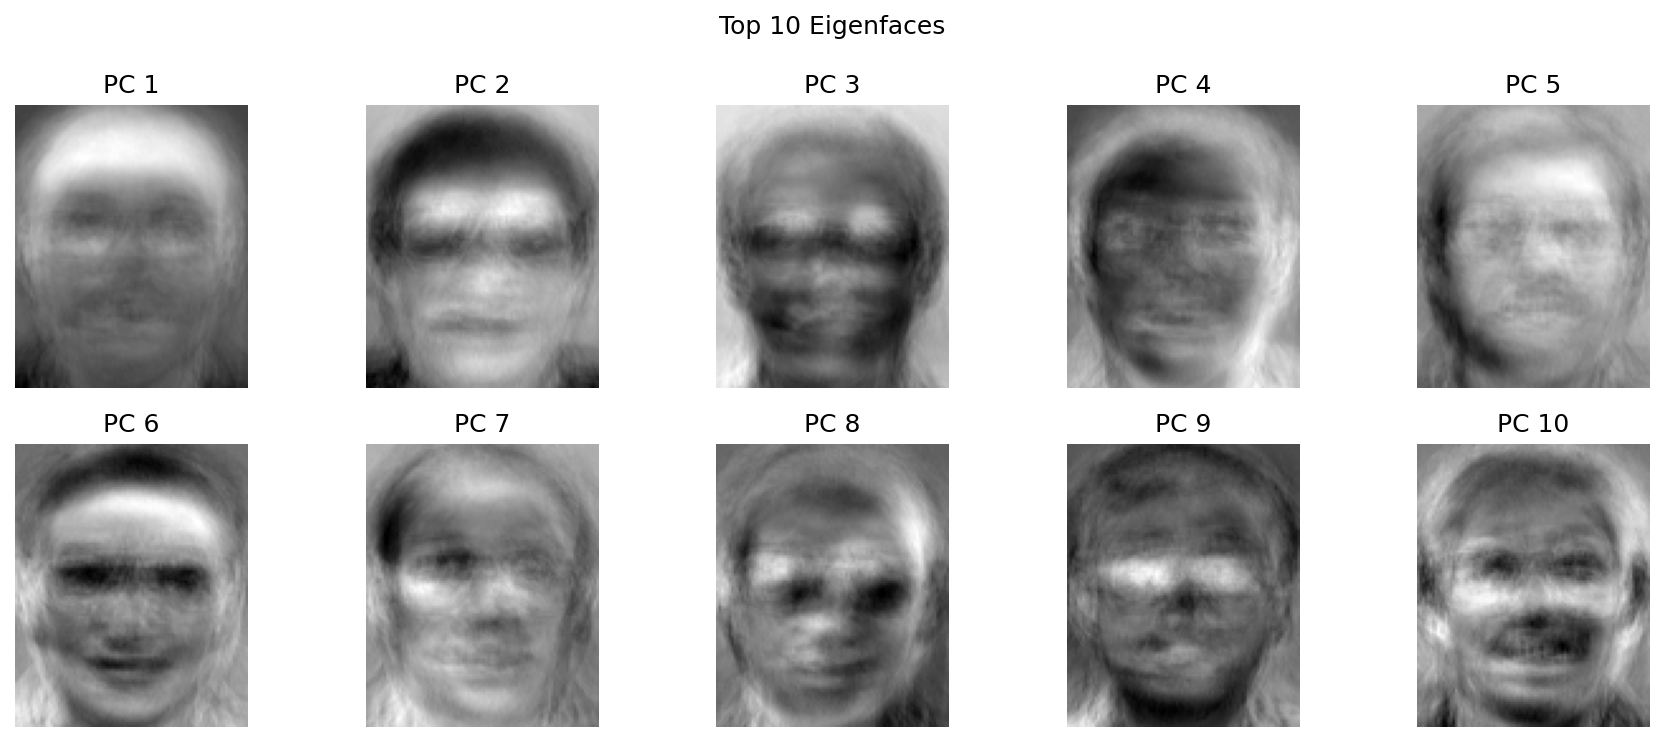
\includegraphics[width=0.9\linewidth]{figures/eigenfaces.png}
    \caption{Top eigenfaces (principal components) learned from the training set.}
    \label{fig:eigenfaces}
\end{figure}

\begin{figure}[H]
    \centering
    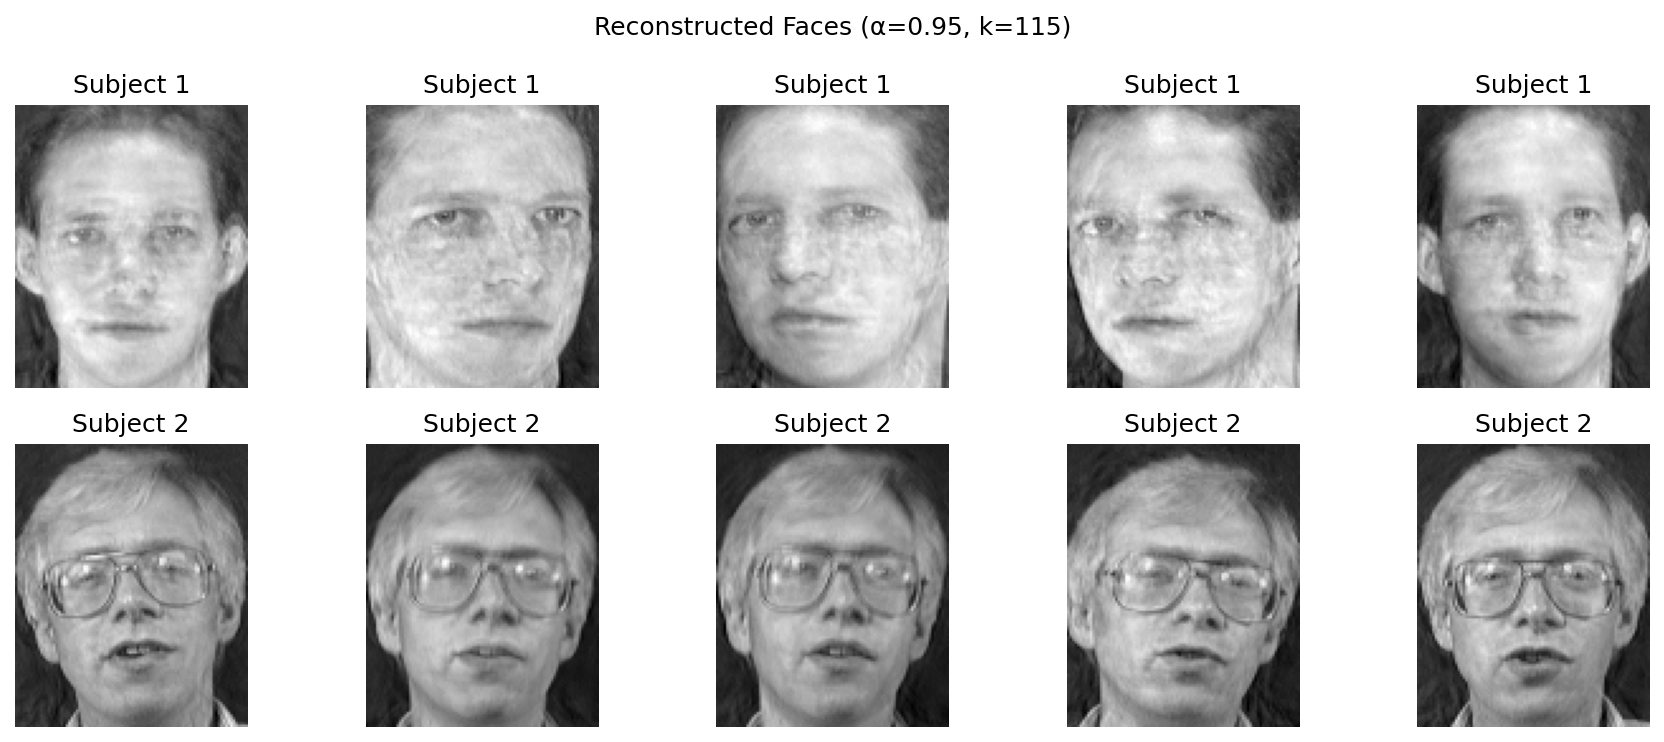
\includegraphics[width=0.9\linewidth]{figures/reconstructions.png}
    \caption{Example reconstructions from the PCA subspace for a chosen $\alpha$. Larger $\alpha$ typically improves reconstruction quality because more components are retained.}
    \label{fig:recon}
\end{figure}

\subsection{K-Means: Accuracy vs $K$ and $\alpha$}
\begin{figure}[H]
    \centering
    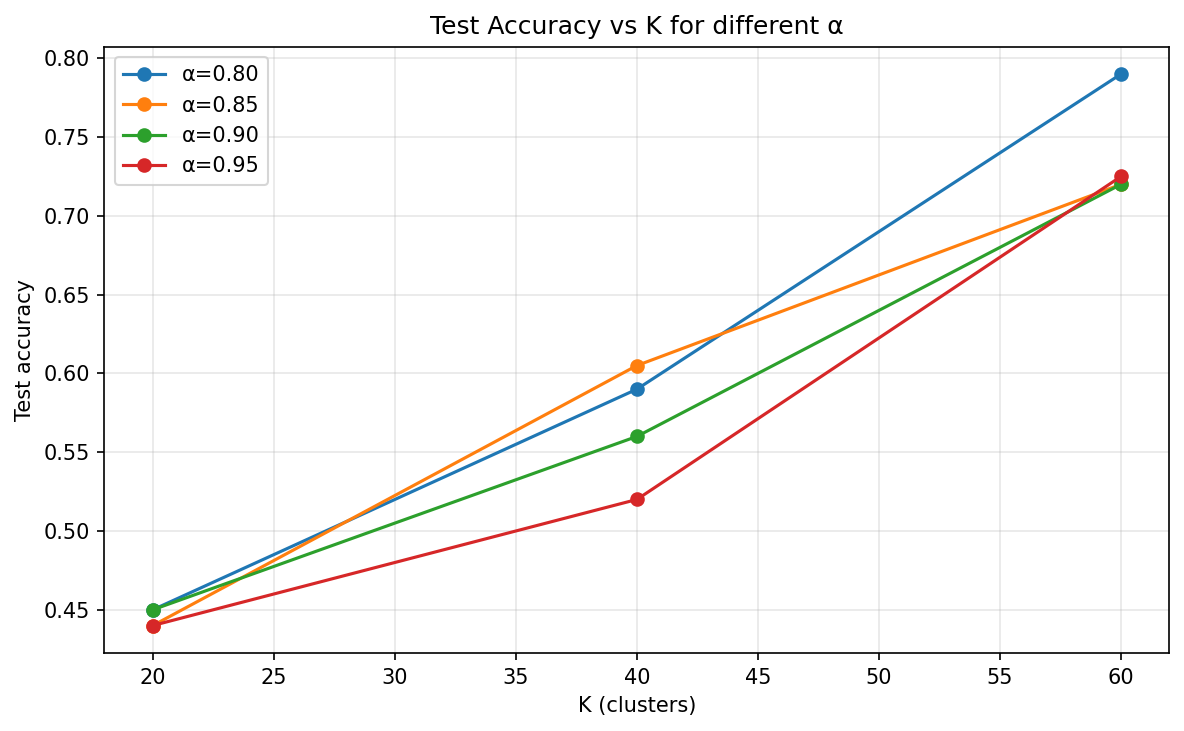
\includegraphics[width=0.8\linewidth]{figures/kmeans_acc_vs_k.png}
    \caption{K-Means test accuracy vs number of clusters $K$, with one curve per $\alpha$.}
    \label{fig:kmeans-k}
\end{figure}

\begin{figure}[H]
    \centering
    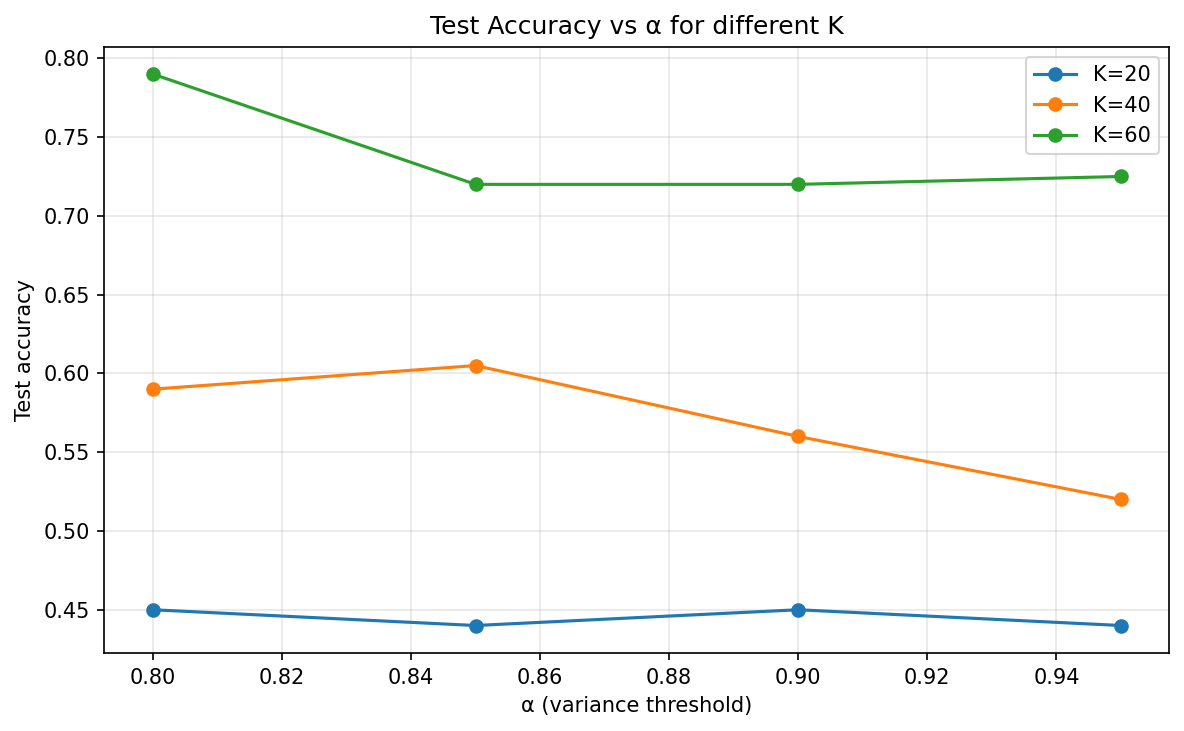
\includegraphics[width=0.8\linewidth]{figures/kmeans_acc_vs_alpha.png}
    \caption{K-Means test accuracy vs variance threshold $\alpha$, with one curve per $K$.}
    \label{fig:kmeans-alpha}
\end{figure}

\subsection{GMM: Accuracy vs $K$ and $\alpha$}
\begin{figure}[H]
    \centering
    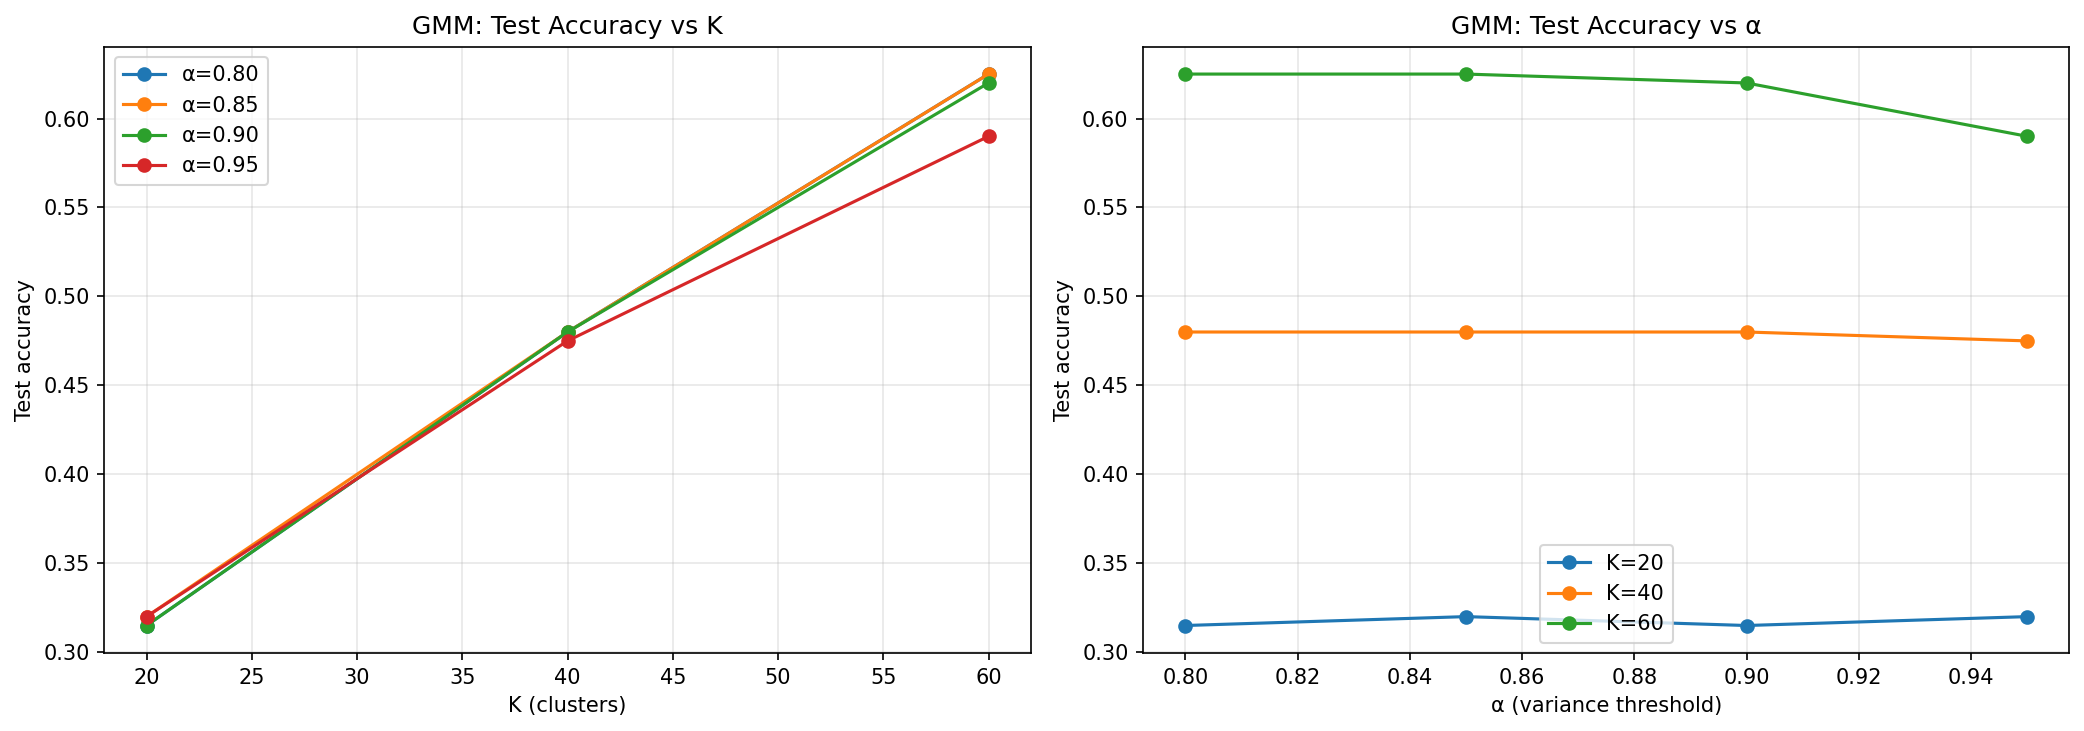
\includegraphics[width=0.8\linewidth]{figures/gmm_acc_vs_k.png}
    \caption{GMM test accuracy vs $K$ (one curve per $\alpha$).}
    \label{fig:gmm-k}
\end{figure}

\begin{figure}[H]
    \centering
    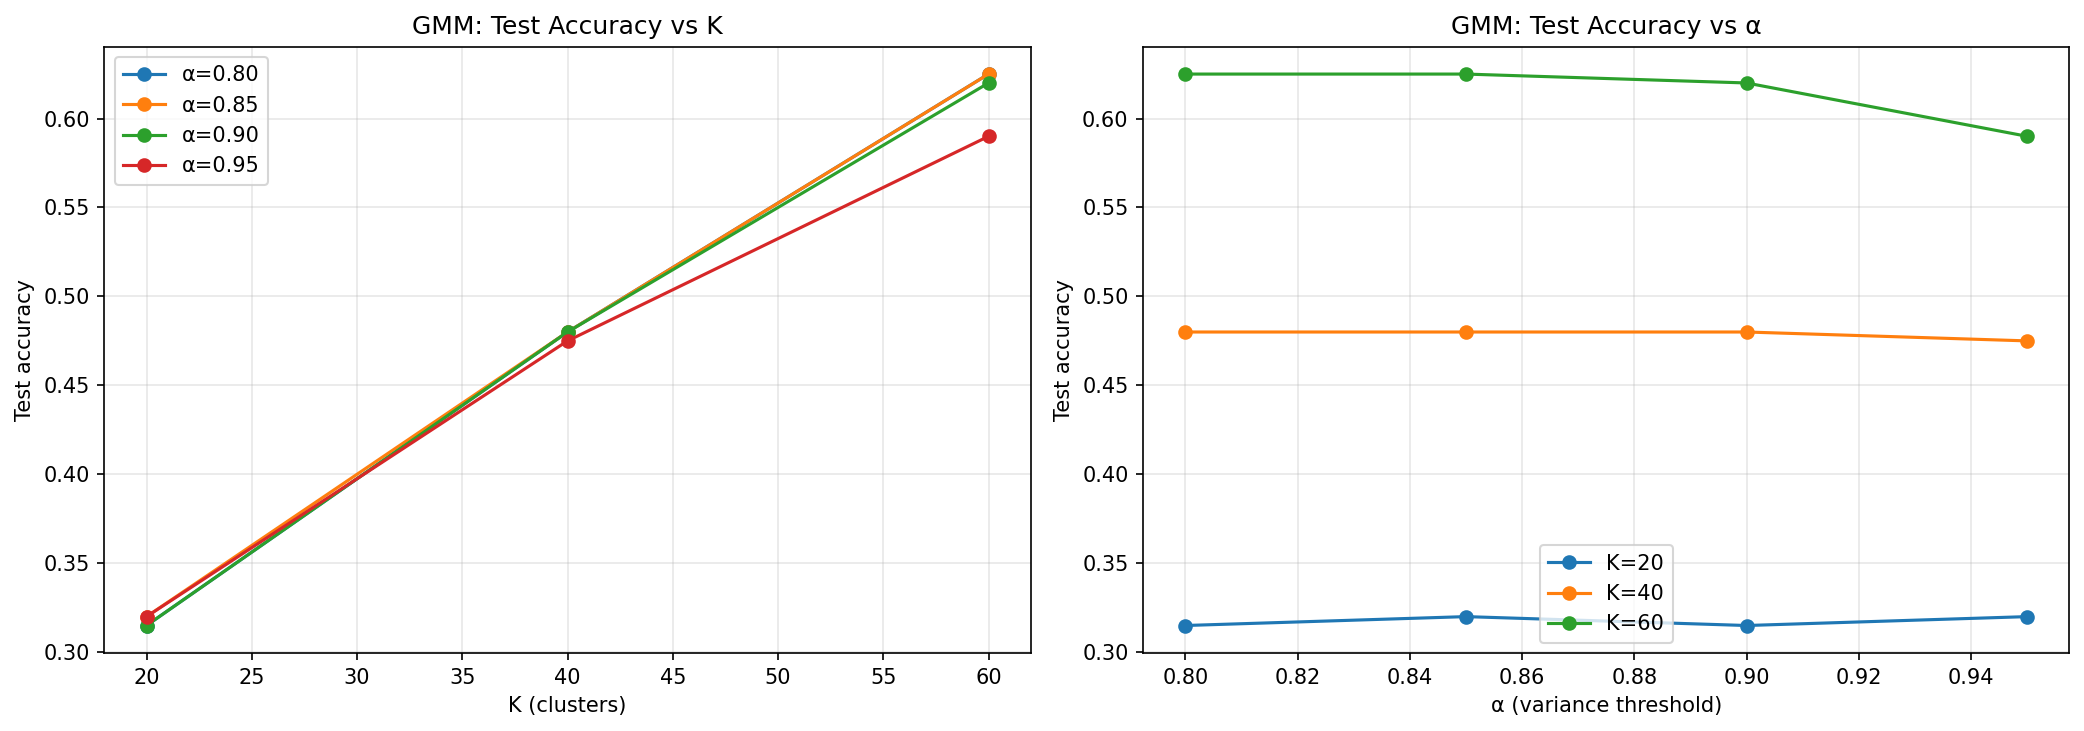
\includegraphics[width=0.8\linewidth]{figures/gmm_acc_vs_alpha.png}
    \caption{GMM test accuracy vs $\alpha$ (one curve per $K$).}
    \label{fig:gmm-alpha}
\end{figure}

\subsection{Confusion Matrices for Best Configurations}
We select the best hyperparameters $(\alpha, K)$ using training accuracy, then report test performance including confusion matrices.

\begin{figure}[H]
    \centering
    \begin{subfigure}{0.48\linewidth}
        \centering
        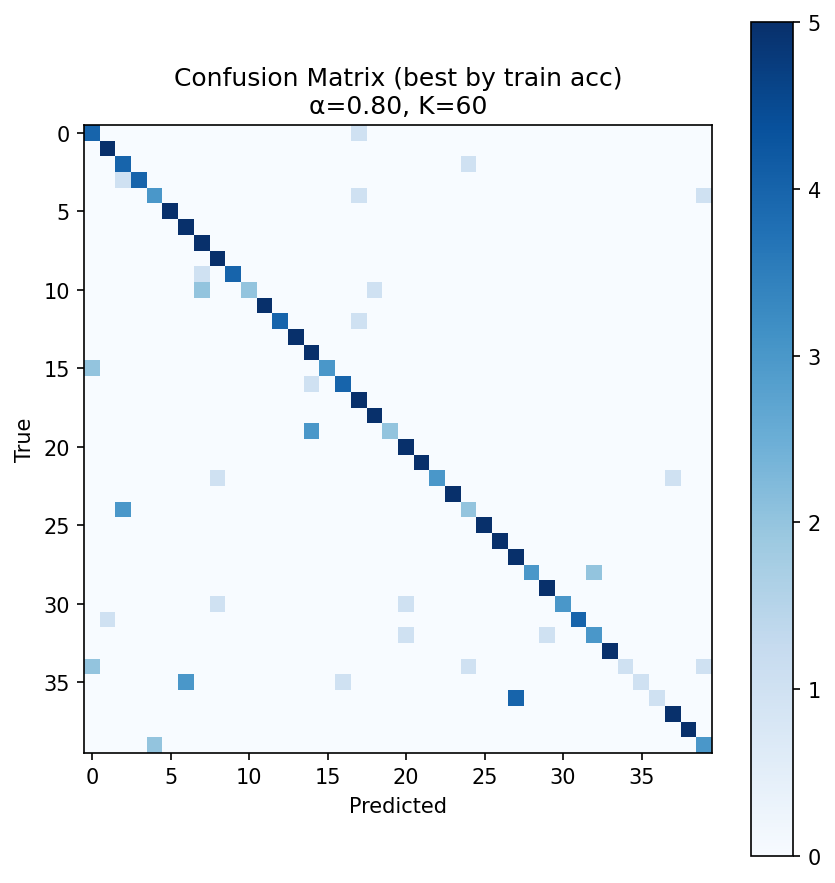
\includegraphics[width=\linewidth]{figures/cm_kmeans.png}
        \caption{K-Means confusion matrix (test).}
    \end{subfigure}
    \hfill
    \begin{subfigure}{0.48\linewidth}
        \centering
        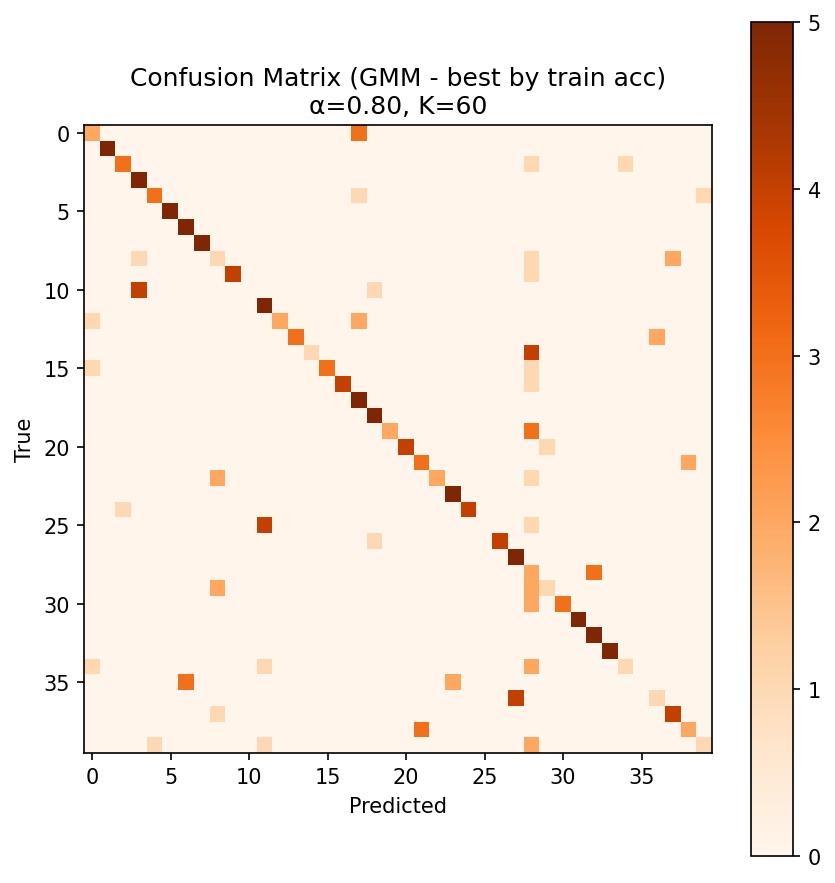
\includegraphics[width=\linewidth]{figures/cm_gmm.png}
        \caption{GMM confusion matrix (test).}
    \end{subfigure}
    \caption{Test-set confusion matrices for the best configuration selected on training accuracy.}
    \label{fig:cms}
\end{figure}

\subsection{Relationship Between $\alpha$ and Classification Accuracy}
\textbf{Trend (expected/typical):}
\begin{itemize}
    \item Increasing $\alpha$ increases the number of retained PCA components $k$, which usually captures more identity-relevant information and can improve clustering/classification accuracy up to a point.
    \item However, very large $\alpha$ may start including components dominated by noise, illumination changes, or background variation. This can reduce cluster separability and may slightly decrease accuracy (diminishing returns).
\end{itemize}

\textbf{How to conclude from your plots:}
Use Figure~\ref{fig:kmeans-alpha} and Figure~\ref{fig:gmm-alpha} to observe whether accuracy increases monotonically with $\alpha$ or peaks at an intermediate value. If accuracy peaks at e.g. $\alpha=0.90$ and then saturates or declines, the relationship is \emph{non-linear} with diminishing returns.

\subsection{Relationship Between $K$ and Classification Accuracy}
\textbf{Trend (expected/typical):}
\begin{itemize}
    \item If $K$ is too small, multiple subjects are forced into the same cluster (under-clustering), lowering accuracy.
    \item If $K$ is too large, a single subject may be split into multiple clusters (over-clustering); after label-mapping, these extra clusters can cause inconsistent predictions and reduce generalization.
\end{itemize}

\textbf{Interpretation for this lab:}
Since the dataset contains multiple subjects (often 40 subjects in the classic ORL/ATT set), accuracy is often higher when $K$ is close to the true number of classes. Therefore, accuracy may improve as $K$ moves toward that value and then stabilize or decline if $K$ exceeds it.

\section{Model Comparison: K-Means vs GMM}
\begin{itemize}
    \item \textbf{K-Means} assumes spherical clusters and optimizes only the centroid positions. It is fast and stable but limited when clusters have different shapes/variances.
    \item \textbf{GMM} is more flexible because each component has a mean and covariance (elliptical clusters), which can better model variations in face space after PCA.
\end{itemize}

\textbf{Comparison criteria:}
\begin{enumerate}
    \item Best achieved test accuracy / weighted F1.
    \item Stability across hyperparameters (how sensitive to $\alpha$ and $K$).
    \item Confusion matrices: which subjects are systematically confused.
\end{enumerate}

\section{Conclusion}
PCA provides an effective compact representation for face images. The variance threshold $\alpha$ controls the retained information and strongly affects clustering separability. The number of clusters $K$ also impacts performance, with best results usually around the true number of identities. Overall, GMM can outperform K-Means when class clusters have different covariances, but the final conclusion should be taken from the reported metrics and plots.

\section*{How to Produce the Figures}
Export the following plots from your notebook into \texttt{figures/} with these filenames:
\begin{itemize}
    \item \texttt{eigenfaces.png}, \texttt{reconstructions.png}
    \item \texttt{kmeans\_acc\_vs\_k.png}, \texttt{kmeans\_acc\_vs\_alpha.png}
    \item \texttt{gmm\_acc\_vs\_k.png}, \texttt{gmm\_acc\_vs\_alpha.png}
    \item \texttt{cm\_kmeans.png}, \texttt{cm\_gmm.png}
\end{itemize}

\end{document}

